\section*{Úkol 1}
\label{sec:task-1}

Pomocí nástrojů explorační analýzy zkoumejte nárůst výkonnostních skóre (FPS) po aplikaci 1.5 patche 
(tj. rozdíl výkonnostních skóre pro verzi „patched“ a verzi „release“) ve hře "Cyberpunk 2077" pro grafické karty 
Nvidia RTX 3070 Ti a AMD Radeon RX 7700 XT. Data vhodně graficky prezentujte (krabicový graf, histogram, q-q graf) 
a doplňte následující tabulku a text.

\vspace{2em}
\noindent
Výsledky popisné statistiky lze vidět v \tabref{tab:characteristics-summary} a na \figref{fig:hist_boxplot} a \figref{fig:qq}.

% Fill your table values here :)
\newcommand{\rangeValues}       {70,        59,         69,         58}
\newcommand{\minValues}         {-4.8,      4.2,        5.1,        4.2}
\newcommand{\QfValues}          {5.425,     4.900,      5.500,      4.900}
\newcommand{\medianValues}      {5.700,     5.300,      5.700,      5.300}
\newcommand{\meanValues}        {5.600,     5.371,      5.750,      5.191}
\newcommand{\QtValues}          {6.100,     5.550,      6.100,      5.500}
\newcommand{\maxValues}         {6.6,       15.8,       6.6,        5.9}
\newcommand{\sdValues}          {1.334,     1.452,      0.439,      0.451}
\newcommand{\cvValues}          {23.8,      27.0,       7.6,        8.7}
\newcommand{\skewnessValues}    {-6.9,      6.4,        0.2,        -0.4}
\newcommand{\kurtosisValues}    {51.3,      43.8,       -1.0,       -0.7}
\newcommand{\lowerBoundValues}  {4.4125,    3.9250,     0,          0}
\newcommand{\upperBoundValues}  {7.1125,    6.5250,     0,          0}

% Additional values
\newcommand{\sigmaValues} {2.757, 8.768, 1.997, 8.453}

% Helper command to put everything in table.
\newcommand{\tableValue}[2]{%
    \pgfmathparse{{#1}[#2]}%
    \mbox{\pgfmathresult}%
}

\begin{table}[h!]
    \caption{Nárůst výkonnostních skóre (FPS) po aplikaci 1.5 patche ve hře "Cyberpunk 2077" pro grafické karty Nvidia RTX 3070 Ti a AMD Radeon RX 7700 XT (souhrnné statistiky)}
    \label{tab:characteristics-summary}
    \vspace{0.5em}
    \renewcommand{\arraystretch}{1.3}
    \resizebox{\textwidth}{!}{%
        \begin{tabular}{|p{3.5cm}|P{3cm}|P{3cm}|P{3cm}|P{3cm}|}
            \hline
            & \multicolumn{2}{P{6cm}|}{\textbf{Původní data}} & \multicolumn{2}{P{6cm}|}{\textbf{Data po odstranění odlehlých pozorování}} \\ \hline
            & \centering \textbf{Nvidia RTX 3070 Ti} & \textbf{AMD Radeon RX 7700 XT} & \centering \textbf{Nvidia RTX 3070 Ti} & \textbf{AMD Radeon RX 7700 XT} \\ \hline
            rozsah souboru        & \tableValue{\rangeValues}{0}    & \tableValue{\rangeValues}{1}    & \tableValue{\rangeValues}{2}    & \tableValue{\rangeValues}{3}    \\ \hline
            minimum               & \tableValue{\minValues}{0}      & \tableValue{\minValues}{1}      & \tableValue{\minValues}{2}      & \tableValue{\minValues}{3}      \\ \hline
            dolní kvartil         & \tableValue{\QfValues}{0}       & \tableValue{\QfValues}{1}       & \tableValue{\QfValues}{2}       & \tableValue{\QfValues}{3}       \\ \hline
            medián                & \tableValue{\medianValues}{0}   & \tableValue{\medianValues}{1}   & \tableValue{\medianValues}{2}   & \tableValue{\medianValues}{3}   \\ \hline
            průměr                & \tableValue{\meanValues}{0}     & \tableValue{\meanValues}{1}     & \tableValue{\meanValues}{2}     & \tableValue{\meanValues}{3}     \\ \hline
            horní kvartil         & \tableValue{\QtValues}{0}       & \tableValue{\QtValues}{1}       & \tableValue{\QtValues}{2}       & \tableValue{\QtValues}{3}       \\ \hline
            maximum               & \tableValue{\maxValues}{0}      & \tableValue{\maxValues}{1}      & \tableValue{\maxValues}{2}      & \tableValue{\maxValues}{3}      \\ \hline
            směrodat. odchylka    & \tableValue{\sdValues}{0}       & \tableValue{\sdValues}{1}       & \tableValue{\sdValues}{2}       & \tableValue{\sdValues}{3}       \\ \hline
            variační koefi. (\%)  & \tableValue{\cvValues}{0}       & \tableValue{\cvValues}{1}       & \tableValue{\cvValues}{2}       & \tableValue{\cvValues}{3}       \\ \hline
            šikmost               & \tableValue{\skewnessValues}{0} & \tableValue{\skewnessValues}{1} & \tableValue{\skewnessValues}{2} & \tableValue{\skewnessValues}{3} \\ \hline
            špičatost             & \tableValue{\kurtosisValues}{0} & \tableValue{\kurtosisValues}{1} & \tableValue{\kurtosisValues}{2} & \tableValue{\kurtosisValues}{3} \\ \hline
            \multicolumn{5}{|p{16cm}|}{\textbf{Identifikace odlehlých pozorování (vnitřní hradby)}} \\ \hline
            dolní mez   & \tableValue{\lowerBoundValues}{0} & \tableValue{\lowerBoundValues}{1} & \multicolumn{2}{P{6cm}|}{------------} \\ \hline
            horní mez   & \tableValue{\upperBoundValues}{0} & \tableValue{\upperBoundValues}{1} & \multicolumn{2}{P{6cm}|}{------------} \\ \hline
        \end{tabular}%
    }
\end{table}

\newpage
\noindent
\textbf{Grafická prezentace (krabicový graf, histogram, q-q graf)}

\begin{figure}[h!]
    \centering
    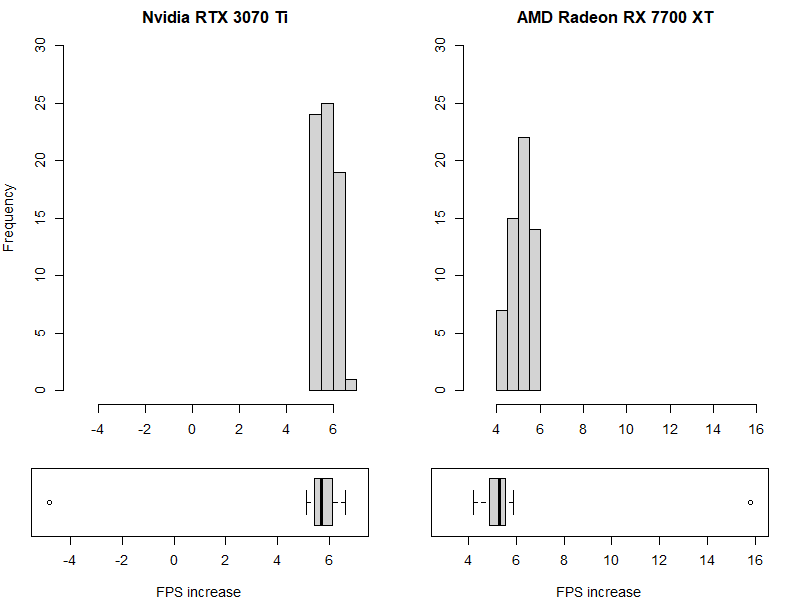
\includegraphics[width=0.85\textwidth]{assets/hist_boxplot}
    \caption{Krabicový graf a histogram znázorňující rozložení nárůstu FPS po aplikaci 1.5 patche ve hře "Cyberpunk 2077" pro grafické karty Nvidia RTX 3070 Ti a AMD Radeon RX 7700 XT}
    \label{fig:hist_boxplot}
\end{figure}

\begin{figure}[h!]
    \centering
    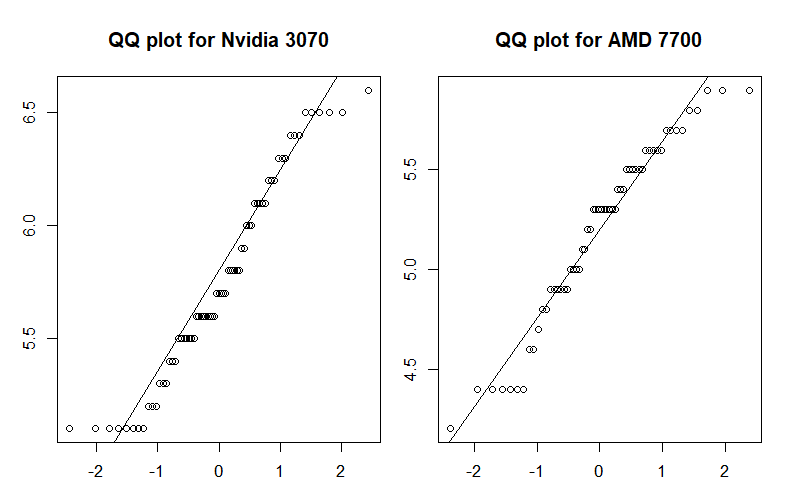
\includegraphics[width=0.8\textwidth]{assets/qq}
    \caption{Q-Q graf znázorňující nárůst FPS po aplikaci 1.5 patche ve hře "Cyberpunk 2077" pro grafické karty Nvidia RTX 3070 Ti a AMD Radeon RX 7700 XT}
    \label{fig:qq}
\end{figure}

\newpage
\subsubsection*{Analýza nárůstu výkonnostních skóre (FPS) po aplikaci 1.5 patche ve hře "Cyberpunk 2077" pro grafickou kartu Nvidia RTX 3070 Ti}

% TODO: Solve underline questions.
Během testu byl zjišťován nárůst FPS pro grafickou kartu Nvidia RTX 3070 Ti ve hře "Cyberpunk 2077" mezi původním release a verzí s 1.5 patchem 
pro \tableValue{\rangeValues}{0} testovacích systémů. Zjištěný nárůst FPS se pohyboval v rozmezí \tableValue{\minValues}{0} FPS
až \tableValue{\maxValues}{0} FPS. \ul{Nárůst FPS v testu č. 20 byl na základě metody vnitřních hradeb identifikován jako odlehlé pozorování
a nebude zahrnut do dalšího zpracování. \footnote{V případě potřeby (existence vícero odlehlých pozorování) větu vhodným způsobem upravte.}
Možné příčiny vzniku odlehlých pozorování jsou: Chyba při testování vzklá náhlým výkyvem výkonem počítače.} Dále uvedené výsledky tedy pocházejí z
analýzy nárůstů FPS zjištěných u \tableValue{\rangeValues}{2} testovacích systémů. Průměrný nárůst FPS byl \tableValue{\meanValues}{2} FPS,
směrodatná odchylka pak \tableValue{\sdValues}{2} FPS. U poloviny testovacích cyklů nárůst FPS nepřekročil \tableValue{\medianValues}{2} FPS\@.
V polovině případů se nárůst FPS pohyboval v rozmezí \tableValue{\QfValues}{2} FPS až \tableValue{\QtValues}{2} FPS. \ul{Vzhledem k hodnotě
variačního koeficientu (\mbox{\tableValue{\cvValues}{3}}\%) lze / nelze analyzovaný soubor považovat za homogenní./ Vzhledem k povaze měřené
veličiny není variační koeficient vhodnou mírou pro posouzení variability souboru.}

\vspace{1em}
\noindent
Výsledky pro grafickou kartu AMD Radeon RX 7700 XT lze komentovat obdobně.

\subsubsection*{Ověření normality nárůstu výkonnostních skóre (FPS) po aplikaci 1.5 patche ve hře "Cyberpunk 2077" pro grafickou kartu Nvidia RTX 3070 Ti}

% TODO: Solve underline questions.
Na základě grafického zobrazení (viz \figref{fig:qq}) a výběrové šikmosti a špičatosti (viz \tabref{tab:characteristics-summary}, výběrová šikmost a špičatost \ul{leží \slash neleží}
v intervalu (-2, 2)) \ul{lze \slash nelze} předpokládat, že pozorovaný nárůst FPS má normální rozdělení. Dle \ul{pravidla 3$\sigma$ \slash Čebyševovy nerovnosti}
lze tedy očekávat, že \ul{přibližně u 95 \% \slash alespoň 75 \%} naměřených nárůstů ve výkonu bude \tableValue{\sigmaValues}{0} FPS až \tableValue{\sigmaValues}{1} FPS\@.

\subsubsection*{Ověření normality nárůstu výkonnostních skóre (FPS) po aplikaci 1.5 patche ve hře "Cyberpunk 2077" pro grafickou kartu AMD Radeon RX 7700 XT}

% TODO: Solve underline questions.
Na základě grafického zobrazení (viz \figref{fig:qq}) a výběrové šikmosti a špičatosti (viz \tabref{tab:characteristics-summary}, výběrová šikmost a špičatost \ul{leží \slash neleží}
v intervalu (-2, 2)) \ul{lze \slash nelze} předpokládat, že pozorovaný nárůst FPS má normální rozdělení. Dle \ul{pravidla 3$\sigma$ \slash Čebyševovy nerovnosti}
lze tedy očekávat, že \ul{přibližně u 95 \% \slash alespoň 75 \%} naměřených nárůstů ve výkonu bude \tableValue{\sigmaValues}{2} FPS až \tableValue{\sigmaValues}{3} FPS\@.

\endinput